% !TEX root = /home/carlo/Dokumente/Studium/FP/V64_Interferometrie/main.tex

\section{Theorie}
\subsection{Mathematische Beschreibung der Interferenz}

Das in diesem Versuch verwendete, monochromatische Laserlicht kann als elektromagnetische Welle
beschrieben werden. Der elektrische Wellenanteil des Lichtes kann also durch die in
Gleichung~\eqref{eq:welle} angegebene Funktion von Raum und Zeit mathematisch ausgedrückt werden. Der Vektor $\vec{E_0}$ gibt dabei die Polarisation des Lichtes an.

\begin{equation}
	\vec{E}(\vec{r},t) = \vec{E_0}\cdot \exp i(\omega t - \vec{k}\vec{r})
\label{eq:welle}
\end{equation}

Der verwendete HeNe-Laser liefert kohärentes, also interferenzfähiges Licht. Bei der Interferenz
addieren sich die elektrischen Feldstärken zweier elektromagnetischen Wellen in jedem Raumzeitpunkt, sodass eine überlagerte Welle entsteht. Die beiden Wellen werden demnach wie folgt beschrieben, wobei die zweite Welle im Vergleich zur ersten eine Phasenverschiebung von $\phi$ besitze und der Winkel zwischen den beiden Polarisationsachsen $\vec{E}_{01}$ und $\vec{E}_{02}$ mit $\delta$ bezeichnet werde:

\begin{align}
\vec{E_1} &= \vec{E}_{01}\cdot \exp i(\omega t - \vec{k}\vec{r}),\\
\vec{E}_2 &= \vec{E}_{02}\cdot \exp i(\omega t - \vec{k} \vec{r} + \phi).
\end{align}

Die beobachtete Intensität ergibt sich also zu

\begin{equation}
I \propto \left<\left|\vec{E}_1+\vec{E}_2\right|^2\right>
=E_{01}^2 + E_{02}^2 + 2E_{01}E_{02}\cos\delta \cos\phi.
\label{eq:intense}
\end{equation}

Bei gleicher Polarisation, also bei $\delta = 0$, sind die Fälle der destruktiven und konstruktiven Interferenz leicht zu identifizieren:

\begin{align}
\phi &= \pi : I\propto E_{01}^2 + E_{02}^2 - 2E_{01}E_{02}
= 0 &\text{ für } E_{01}=E_{02}\\
\phi &= 0 : I\propto E_{01}^2 + E_{02}^2 + 2E_{01}E_{02}
= 4E_{01}^2 &\text{ für } E_{01}=E_{02}
\end{align}

Stehen die Polarisationsrichtungen der beiden Wellen hingegen senkrecht aufeinander, ist also $\delta = \pi/2$, so ergibt sich

\begin{equation}
I \propto E_{01}^2 + E_{02}^2.
\end{equation}

Bei senkrecht zueinander polarisierten Wellen tauchen also keine Interferenzeffekte auf.


\subsection{Kontrast des Interferometers}
Eine wichtige Größe eines Interferometers ist dessen Kontrast $K$. Dieser gibt die auf den Bereich zwischen 0\% und 100\% normierte Differenz zwischen der maximal und minimal einstellbaren Intensität des Lichtstrahls an, welcher aus dem Interferometer heraustritt. Der Kontrast kann durch Gleichung~\eqref{eq:kontrast} definiert werden.

\begin{equation}
K = \frac{I_\text{max}-I_\text{min}}{I_\text{max}+I_\text{min}} \in [0,1]
\label{eq:kontrast}
\end{equation}

Zur Kontrastmessung werden in diesem Versuch zwei Polarisationsfilter verwendet. Der erste lässt nur den Anteil des Lichtes hindurch, welcher im Winkel $\theta$ zur horizontalen Achse liegt. Dadurch gilt für die Beträge der beiden Teilstrahlen, welche durch den PBSC entstehen, folgender Zusammenhang:

\begin{align*}
E_{01}=E\cdot\cos \theta,\\
E_{02}=E\cdot\sin \theta.
\end{align*}

Der zweite Filter lässt von beiden senkrecht zueinander polarisierten Strahlen nur jeweils die Komponenten der elektrischen Felder durch, welche parallel zur Polarisationsrichtung des Filters stehen, sodass beide Teilstrahlen anschließend die gleiche Polarisationsrichtung aufweisen und der Winkel $\delta$ zwischen den beiden Polarisationsvektoren verschwindet.


Eingesetzt ergibt sich also für die Intensität des Lichtes am Ende des Interferometers in Abhängigkeit des
eingestellten Winkels des ersten Polarisationsfilters der in Formel~\eqref{eq:kontrastwinkel} angegebene Zusammenhang.

\begin{equation}
I \propto E^2\cdot(1 + 2\cos \theta \sin \theta \cos \phi)
\label{eq:kontrastwinkel}
\end{equation}

Für den Phasenunterschied $\phi = 0$ ergibt sich die maximale Intensität

\begin{equation}
I_\text{max} \propto E^2\cdot(1 + 2\cos \theta \sin \theta).
\label{eq:intens_max}
\end{equation}

Die minimale Intensität folgt für $\phi = \pi$ zu

\begin{equation}
I_\text{min} \propto E^2\cdot(1 - 2\cos \theta \sin \theta).
\label{eq:intens_min}
\end{equation}

Für den Kontrast gilt also in Abhängigkeit vom eingestellten Winkel $\theta$ des Polarisationsfilters der in Gleichung \eqref{eq:kontr} beschriebene Zusammenhang. Für $\theta = 0$ und $\theta = \pi/2$ sind $I_\text{min}$ und $I_\text{max}$ identisch und bei $\theta = \pi/4$ liegt ein maximaler Kontrast von 100\% vor.

\begin{equation}
	K = 2 \cos \theta \sin \theta = \sin 2\theta
	\label{eq:kontr}
\end{equation}


\subsection{Brechungsindizes}
Im Vakuum propagiert eine elektromagnetische Welle mit der Lichtgeschwindgkeit $c$, Materie hingegen wird von Licht langsamer durchdrungen. Diese Verlangsamung des Lichtes ist der Grund für das Phänomen der Lichtbrechung. Daher kann der Brechungsindex $n$ wie in Formel~\eqref{eq:brech} angegeben, definiert werden. Dabei bezeichnet $v$ die Materielichtgeschwindigkeit.

\begin{equation}
n = \frac{c}{v}
\label{eq:brech}
\end{equation}

Durch die Verlangsamung des Lichtes in Materie wird dessen Wellenlänge größer und somit dessen Wellenzahl kleiner. Bei eindimensionaler Betrachtung wird die Wellenzahl in Materie zu

\begin{equation*}
k = \frac{2\pi}{\lambda_\text{vac}}n.
\end{equation*}

\paragraph{Brechungsindex von Glasplatten}
\begin{figure}
\centering
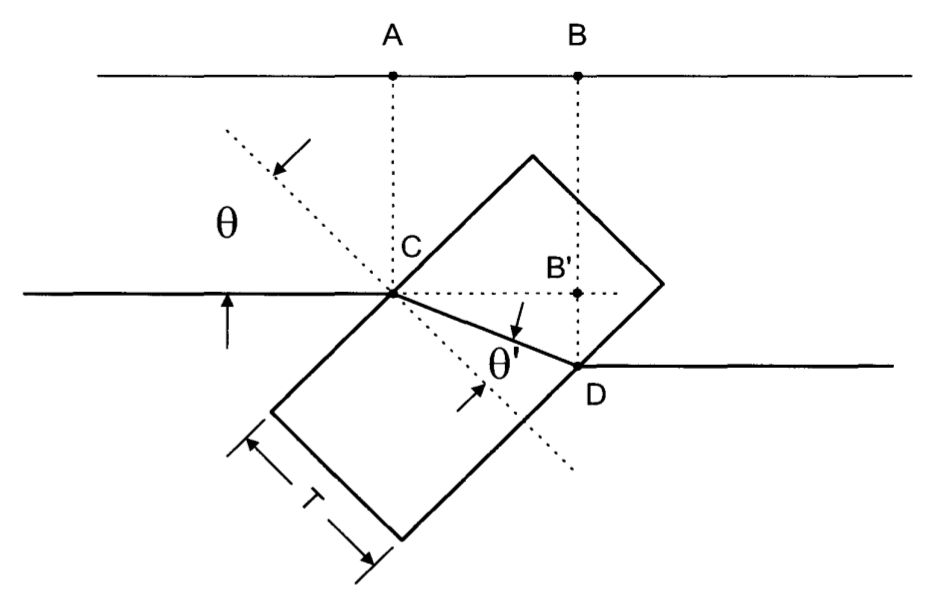
\includegraphics[width=0.7\linewidth]{img/slab.png}
\caption{Darstellung des Strahlengangs bei der Bestimmung des Brechungsindex einer Glasplatte. [Quelle!]}
\label{fig:slab}
\end{figure}

Fällt Licht im Winkel $\Theta$ zum Lot auf eine Glasplatte der Dicke $T$ mit Brechungsindex $n$ und schließt der eingetretene Strahl mit dem Lot den Winkel $\Theta'$ ein, so kann durch das Snelliussche Brechungsgesetz der Phasenunterschied $\phi$ zwischen einem Strahl, der am Glas vorbeiläuft und einem, der durch das Glas hindurchgeht, nach Formel~\eqref{eq:glasbrech} errechnet werden. Abbildung \ref{fig:slab} visualisiert die vorliegende Situation.

\begin{equation}
\Delta\phi(\Theta) = \frac{2\pi}{\lambda_\text{vac}}T\left(
\frac{n-\cos(\Theta - \Theta')}{\cos(\Theta')} - n+1\right)
\label{eq:glasbrech}
\end{equation}

Einsetzen von $\Theta'$ und eine Kleinwinkelnäherung um $\Theta = 0$ ergeben die einfachere Formel~\eqref{eq:glasbrecheinfach}.

\begin{equation}
\Delta\phi(\Theta) = \frac{2\pi T}{\lambda_\text{vac}}
\frac{n-1}{2n}\Theta^2 + \mathcal{O}(\Theta^4)
\label{eq:glasbrecheinfach}
\end{equation}

In diesem Versuch wird die Anzahl $M$ der $2\pi$-Phasenverschiebungen der Strahlen während einer Rotation zweier Glasplatten um den Winkel $\Theta$ gemessen. Diese Anzahl ergibt sich mit Formel~\eqref{eq:glasbrecheinfach} zu

\begin{equation}
M = 2\frac{\Delta\phi}{2\pi} \approx \frac{2T}{\lambda_\text{vac}}
\frac{n-1}{2n}\Theta^2.
\label{eq:glasfringes}
\end{equation}

Aus dieser Formel kann in diesem Versuch der Brechungsindex $n$ von Glasplatten bestimmt werden.

\paragraph{Brechungsindex von Gas}
Durchläuft Licht ein Gas mit dem Brechungsindex $n$ auf einer Strecke $L$, so beträgt der Phasenunterschied zu einem parallel dazu im Vakuum laufenden Strahl

\begin{equation}
\Delta\phi = \frac{2\pi}{\lambda_\text{vac}}(n-1)L.
\end{equation}

Hieraus ergibt sich ein Ausdruck für die Anzahl $M$ der gezählten $2\pi$-Phasen\-ver\-schie\-bung\-en durch Division mit $2\pi$. Also kann mithilfe von Formel~\eqref{eq:gasfringes} der Brechungsindex eines Gases in diesem Versuch bestimmt werden. 

\begin{equation}
M = \frac{\Delta\phi}{2\pi} = \frac{n-1}{\lambda_\text{vac}}\cdot L
\label{eq:gasfringes}
\end{equation}
